\section{Prototipo realizacija}

Šis skyrius aprašo praktinę rašto darbo pusę -- debesų kompiuterijos technologijomis grįstos saityno peržiūros roboto realizacijos sprendimus. Architektūra ir naudojami įrankiai parinkti pagal 4 skyriuje apibrėžtus sistemos reikalavimus.

\subsection{Sistemos panaudojamumas}

Įgyvendinant prototipo architektūrą pagal 4 skyriuje išsikeltus reikalavimus, apibrėžtos pagrindinės veiklos, kurios sudaro sistemos funkcionalumą, jos matomos \ref{fig:use_case_diagram} paveikslėlyje pavaizduotoje UML panaudojamumo diagramoje.

\begin{figure}[htp!]
\centering
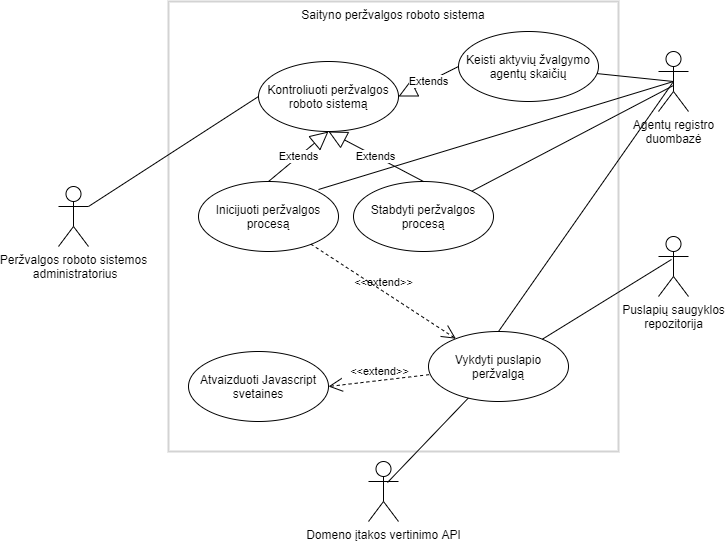
\includegraphics[scale=0.6]{img/Use_case_diagram.png}
\caption{UML žvalgymo roboto sistemos prototipo panaudojamumo diagrama}
\label{fig:use_case_diagram}
\end{figure}

Svarbu paminėti keletą aiškinamųjų aspektų apie diagramoje pavaizduotas veiklas ir aktorius.


\textbf{Peržvalgos roboto sistemos administratorius} -- klientinė programa, kontroliuojanti žvalgymo procesą. Klientas gali būti įvairių formų: komandinės eilutės programa, žiniatinklio, darbalaukio programa. Prototipo realizacijoje klientinė programa imituojama naudojantis \textit{„Service Bus Explorer“\footnote{https://github.com/paolosalvatori/ServiceBusExplorer}} įrankiu ir rankiniu būdu siunčiant žinutes į sistemos žvalgymo kontroliavimo eilę.

\textbf{Domeno įtakos vertinimo API} -- išorinis tarnybos serveris, kuris sugeba skalėje nuo 1 iki 100 įvertinti konkretaus domeno autoritetą, kuris reikalingas žvalgymo prioritizavimui. Prototipo įgyvendinimo metu naudota \textit{openrank.io\footnote{https://openrank.io/}} API paslauga, suteikianti 10000 nemokamų užklausų per 24 valandas. Akcentuotina, kad ši išorinė sistema nėra privaloma -- darbe pasirinkta etiško žvalgymo politika atsižvelgia į šią metriką siekiant nustatyti populiaresnes svetaines, kurias galima žvalgyti greičiau.

\textbf{Atvaizduoti Javascript svetaines} -- šis panaudojamumo atvejis yra vykdomas kaip atskira veikla po peržvalgos proceso, jei konkretus puslapis pasižymi dinaminės svetainės, kuri turinį generuoja klientinėje pusėje, savybėmis.

\subsection{Naudojama architektūra}

Prototipas rengiamas plačiai remiantis Kalifornijos Mersedo universiteto mokslininkų literatūrine medžiaga apie debesų kompiuterijos išskirstyto saityno žvalgymo roboto sistemą ir jos architektūrą, dizaino principus \cite{MercedCloudBasedWebCrawler}. Atsižvelgiant į darbo rašymo metus ir patobulėjusias debesų kompiuterijos tiekėjų siūlomas technologijas, pasiūlyta architektūra realizuojama pritaikius specifinius pokyčius pakeičiant realizacijos įrankius ir platformas.  

\begin{figure}[ht]
\centering
\includegraphics[scale=0.6]{img/Mersed_architektūra.png}
\caption{Mersedo universiteto mokslininkų pasiūlyta saityno peržiūros roboto architektūra \cite{MercedCloudBasedWebCrawler}}
\label{fig:mersed_architecture}
\end{figure}

\subsubsection{Centrinis žvalgymo variklis}
 
 Tai pagrindinis sistemos struktūrinis komponentas, kuris inicijuoja visą žvalgymo procesą ir kuria/naikina žvalgymo agentus. Pagrindiniai šio komponento veikimo etapai:
 \begin{enumerate}
     \item Inicializacija
     \begin{enumerate}
         \item Paimami pradiniai URL adresai iš žvalgymo adresų sąrašo
         \item Adresai sudedami į „Azure“ eilę prieš tai patikrinant, ar kiekvienas URL adresas dar nebuvo žvalgytas ( naudojamas \textit{„Azure NoSQL Table Storage“})
         \item Sukuriamas pirmasis žvalgymo agentas, jam priskiriama jo žvalgymo zona (svetainės serverio vardas)
     \end{enumerate}
     \item Ciklinis žvalgymo procesas
     \begin{enumerate}
         \item Iš žvalgymo eilės paimamas URL adresas
         \item Patikrinama, ar esama adresui egzistuoja aktyvus agentas (SQL Agentų registro duombazė)
         \item Jei agentas egzistuoja, URL adresas ignoruojamas, nes priskirtas agentas jį apdoros
         \item Jei aktyvaus agento nėra, paskaičiavus aktyvių agentų skaičių A\textsubscript{aktyvūs} tikrinamas maksimalus leistinas agentų skaičius A\textsubscript{max} > A\textsubscript{aktyvūs}, jei sąlyga patenkinta, bandoma sukurti naują agentą ir jam priskirti URL adreso vardo zoną. Kitu atveju laukiama, kol sąlyga bus patenkinta (agentai baigs savo darbą).
         \item Kartojama nuo pirmo žingsnio
     \end{enumerate}
 \end{enumerate}
 
 \subsubsection{Žvalgymo agentas}

Šis komponentas iš žvalgymo eilės ima URL adresą, jei adreso vardo sritis sutampa su agentui priskirtu aptarnavimo vardo adresu, jis inicijuoja HTTP užklausą į nurodytą žiniatinklio serverį, parsiunčia HTML turinį, išgauna visas jame esančias nuorodas, kiekvienai jų patikrina, ar nuoroda dar neregistruota indeksų repozitorijoje ir atitinkamai perduoda aktyviam žvalgymo agentui, kurio zona sutampa su URL adreso vardo zona. Agentai užtikrina išskirstytos sistemos veikimo principą, juos dinamiškai galima pridėti, šalinti. Nėra jokio centrinio komunikacijos komponento, kuris deleguotų žvalgymo darbus agentams.

 \subsubsection{Agentų registras}
 
 Tai SQL duombazė, kurioje registruojami visi aktyvūs agentai, taip pat jie periodiškai išregistruojami aptikus, jog agentas kurį laiką nebuvo aktyvus. Šis komponentas yra bendras, todėl rašto darbo paskutiniame skyriuje, atliekant tyrimą, bus analizuojama, ar jis negali lemti „butelio kaklelio“ efekto.
 
 % Table generated by Excel2LaTeX from sheet 'crawling_vs_scraping'
\begin{table}[htbp]
  \centering
  \caption{Agentų registro lentelės schema \cite{MercedCloudBasedWebCrawler}}
    \begin{tabular}{|l|l|l|l|l|}
    \hline
    \textbf{Id} & \textbf{Agento\_Vardas} & \textbf{Agento\_Aptarnavimo\_Sritis} & \textbf{\textcolor{red}{Paskutinis\_Aktyvumas}} & \textbf{Ištrintas} \bigstrut\\
    \hline
    1 & A1 & abc.lt & 2020-05-02 15:30:15 & false \\
    \hline
    2 & A2 & def.lt & 2020-05-02 13:30:15 & true \\
    \hline
    \end{tabular}%
  \label{tab:agent_registry_table}%
\end{table}%
 
 \ref{tab:agent_registry_table} lentelėje pavaizduotoje agentų registro lentelėje raudonai pažymėtas paskutinio aktyvumo laiko stulpelis originaliai \cite{MercedCloudBasedWebCrawler} literatūroje neminėtas, tai -- rašto darbo autoriaus prototipo planavimo metu įgyvendinta korekcija siekiant atlaisvinti nebenaudojamus agentus.
 
 \subsubsection{„Azure“ žvalgymo eilė}
 
 Tai komponentas, kuris saityno žvalgymo sistemų literatūroje minimas kaip „žvalgymo pasienio“ (angl. -- \textit{Crawling Frontier}) komponentas, kuriame laikinai kaupiami žvalgytinų puslapių URL adresai. Žvalgymo agentai ir Centrinis žvalgymo variklis klausosi šios eilės žinučių ir jas apdoroja. Tai dar vienas bendrinis sistemos komponentas, todėl eksperimento metu taip pat bus stebimas jo veikimo pralaidumas. \cite{MercedCloudBasedWebCrawler} moksliniame darbe jau buvo atliktas šio komponento tyrimas ir įsitikinta, kad didinant žinučių kiekio apkrovą, komponento pralaidumas išlieka gana patovus. Naudota „Azure Storage Queues“ eilių paslauga. Šio rašto darbo tyrime bus naudojama kita „Azure“ paslaugų eilių infrastruktūra, todėl taip pat pakartotinai bus stebimas komponento veikimo optimalumas.
 
 \subsubsection{„Azure“ NoSQL indeksų repozitorija}

Tai NoSQL rakto-reikšmės (angl. -- \textit{Key-Value}) tipo saugykla, kurioje agentai registruoja identifikuotus svetainių URL adresus, taip pat keičia tų adresų žvalgymo statusą, aptiktų URL nuorodų paminėjimų skaičių (angl. -- \textit{hit count}.

\subsubsection{„Azure“ didelių objektų saugykla}

Šis komponentas aprašytoje architektūroje atsakingas už didelių multimedijos failų saugojimą -- nuotraukų, vaizdo įrašų, PDF dokumentų ir kitų žiniatinklio resursų, kurie nėra HTML dokumentai. Pasižymi tuo, jog gali talpinti didelius kiekius duomenų.

\subsubsection{Svetainės turinio analizatorius ir dublikatų aptikimas}

Vienas iš minimų sistemos komponentų -- svetainės turinio analizatorius -- semantiškai apdoroja nuskaitytą HTML dokumento turinį siekdamas nustatyti puslapio tematiką, pagrindinius raktinius žodžius, taip pat identifikuoti pasikartojančio, dublikuoto turinio svetaines. Šio prototipo įgyvendinimo ribose nebuvo numatytas semantinis svetainės turinio analizavimas, todėl plačiau šie komponentai aptariami nebus. Prototipo įgyvendinimo ribose nuamtytas tik URL adresų dublikatų aptikimas siekiant išvengti bereikalingos pakartotinės resurso žvalgymo naštos.

\subsubsection{Decentralizuota komunikacija}

Aprašomos saityno peržvalgos roboto sistemos architektūros išskirtinis bruožas lyginant ją su anksčiau nagrinėtomis literatūroje aprašytomis sistemomis -- nepriklausomas agentų veikimas ir apsikeitimas žvalgytinais puslapiais be centrinio darbo koordinavimo komponento \cite{MercedCloudBasedWebCrawler} (centrinis žvalgymo variklis nekoordinuoja darbo, tik valdo agentų gyvavimo ciklą). Šis išskirtinumas leidžia plėsti sistemos žvalgymo pajėgumus pridedant naujus žvalgymo agentus, kurie savo žvalgymo rezultatus gali perduoti kitiems agentams tiesiogiai be tarpinio komponento. Kiekvienas agentas turi priskirtą aiškia žvalgymo zoną (domeną), todėl atlieka tik savo srities žvalgymo atominę operaciją.

\pagebreak

\subsection{Panaudojamumo atvejų dinamika}

Šiame poskyryje detaliau grafiškai pristatomos apibrėžtų panaudojamumo atvejų agloritminės veikimo sekos, kurios perteikiamos UML sekų diagramomis. 

\subsubsection{Inicijuoti peržvalgos procesą}

Žemiau pateiktoje \ref{fig:initiate_crawling_uml_sequence} UML sekos diagramoje pavaizduotas sistemos administratoriaus inicijuojamas žvalgymo pradėjimo procesas, kurio metu pradinis URL adresų sąrašas perkeliamas į žvalgymo pasienio komponentą ir sukuriamas pradinis žvalgymo agentas.
\begin{figure}[ht!]
\centering
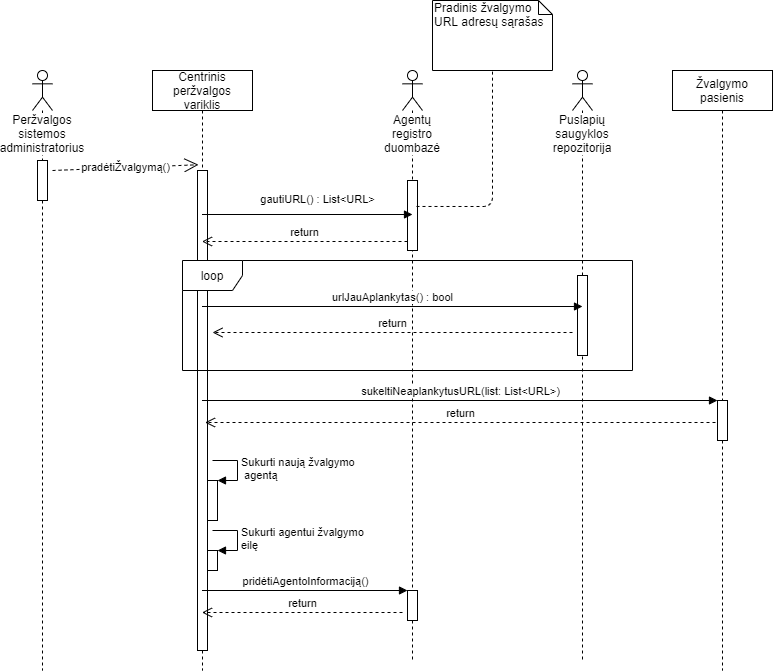
\includegraphics[scale=0.6]{img/initiate_crawling_process_sequence.png}
\caption{Žvalgymo inicijavimo proceso UML sekos diagrama}
\label{fig:initiate_crawling_uml_sequence}
\end{figure}

\pagebreak

\subsubsection{Vykdyti puslapio peržvalgą}

\ref{fig:perform_crawling_uml_sequence} UML sekos diagramoje pavaizduota žvalgymo agento darbo vykdymo schema. Akcentuotina, kad šis žvalgymo procesas kartojamas iki to laiko, kai žvalgymo agento eilė tampa tuščia ir po sistemos konfigūracijoje nustatyto agento neaktyvumo intervalo, Centrinis žvalgymo variklis tiesiog panaikina nebeaktyvų žvalgymo agentą.

\begin{figure}[ht!]
\hspace*{-2cm} 
\centering
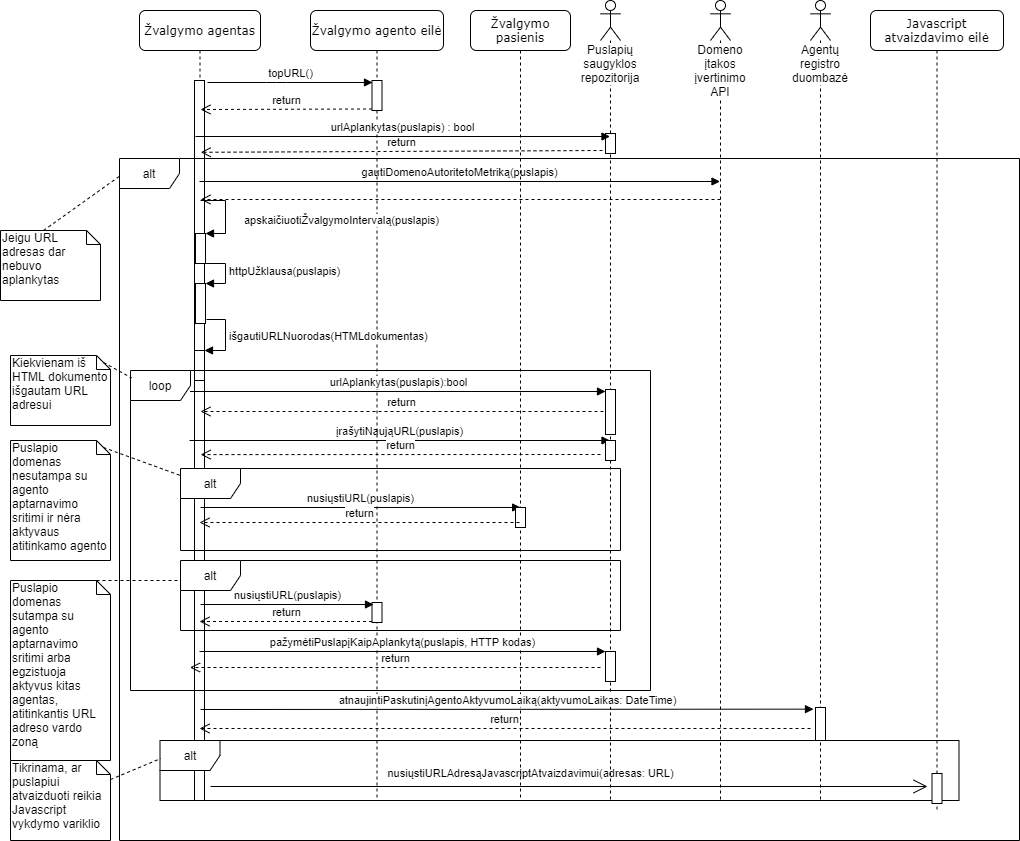
\includegraphics[scale=0.5]{img/perform_cralwing_sequence.png}
\caption{Žvalgymo vykdymo proceso UML sekos diagrama}
\label{fig:perform_crawling_uml_sequence}
\end{figure}

\subsubsection{Poreikis atlikti Javascript atvaizdavimą}

\ref{fig:perform_crawling_uml_sequence} diagramoje paminėta, jog URL adresas po žvalgymo į Javascript atvaizdavimo eilę siunčiamas tik nustačius, jog puslapis reikalauja Javascript atvaizdavimo variklio, kad galėtų dinamiškai generuoti DOM medį. Šiame punkte pateikiama UML veiklos diagrama \ref{fig:js_rendering_condition}, kurioje nurodoma, kaip prototipinė sistema atlieka šį tikrinimą.

\begin{figure}[ht!]
\centering
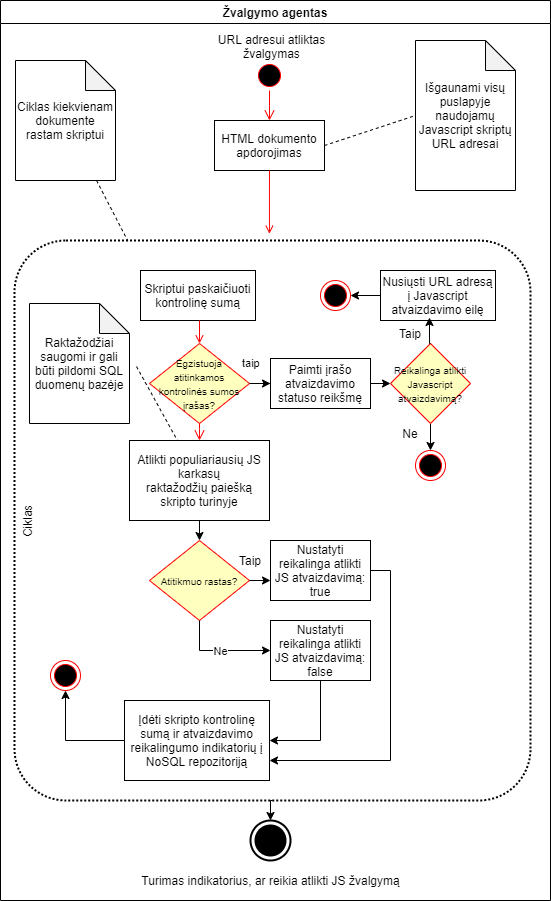
\includegraphics[scale=0.6]{img/javascript_rendering_condition_activity_diagram.png}
\caption{Poreikio atlikti Javascript atvaizdavimą indikatoriaus nustatymo UML veiklos diagrama}
\label{fig:js_rendering_condition}
\end{figure}

\subsection{Struktūrinis prototipo dizainas}

Šiame poskyryje aprašoma koreguota \cite{MercedCloudBasedWebCrawler} mokslininkų pasiūlyta išskirstyto saityno peržvalgos roboto sistemos struktūrinė architektūra. Ji detalizuojama aprašant naudojamas „Microsoft Azure“ debesų kompiuterijos infrastruktūros tiekėjo paslaugas ir resursus. Rašto darbe įgyvendinant prototipą pasirinktas pastarasis debesų kompiuterijos sprendimas dėl rašto darbo autoriaus patirties naudojantis jo paslaugomis, tačiau nėra problemų šią architektūrą realizuoti su bet kuriuo kitu debesų kompiuterijos paslaugų tiekėju (pvz.: Amazon Web Services arba Google Cloud Platform).


Paeiktoje \ref{fig:azure_implementation_structural_scheme} schemoje detalizuojami esminiai sistemos struktūriniai komponentai ir jų „Azure“ platformos infrastruktūros paslaugų rūšys.

\begin{figure}[htp!]
\centering
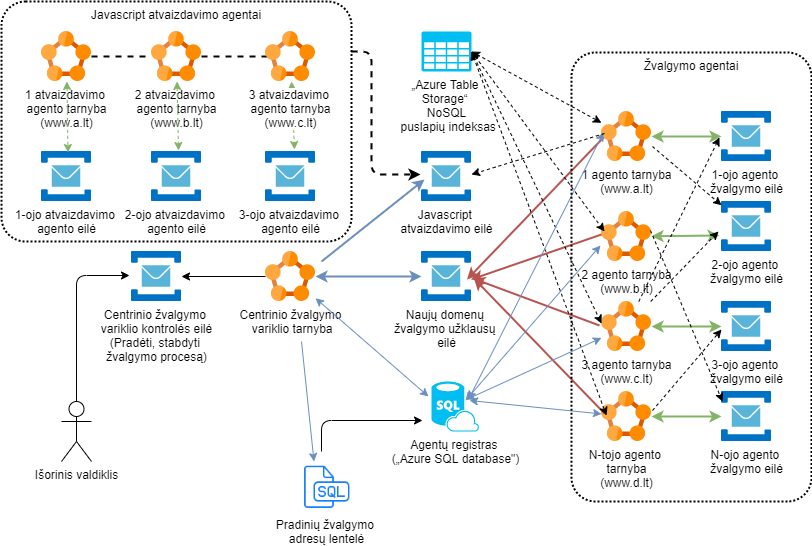
\includegraphics[scale=0.6]{img/Azure_Implementacija_Kasparo.png}
\caption{Struktūrinė prototipo sistemos schema}
\label{fig:azure_implementation_structural_scheme}
\end{figure}



\subsubsection{Žvalgymo agentai}

//TODO aprašyti žvalgymo agentus kaip Service Fabric Stateless Services, paaiškinti, kaip jie komunikuoja su atitinkamomis eilėmis

\subsubsubsection{„Azure Service Bus“ eilės}

//TODO aprašyti žvalgymo, centrinio žvalgymo tarnybos, atvaizdavimo eiles, taip pat naujų domenų žvalgymo užklausų eilę.

\subsubsection{„Azure Table Storage“ indekso saugyklos struktūra}

\subsubsection{Kiti prototipo realizacijoje panaudoti įrankiai}

// TODO: .NET Core 3.1, Dapper, C\# AbotCrawler biblioteka žiniatinklio žvalgymui